\section{Others}

\subsection{Performance Metrics} 

\subsection{Bias vs Variance}

El dilema de \textit{Bias vs Variance} describe la relación entre la complejidad del modelo, la precisión de las predicciones y cómo éste se comporta al predecir datos nunca antes vistos. El error estimado de una predicción viene dado en términos generales por 
$$
\text{Expected Error} = (\text{Bias})^2 + \text{Variance} + \text{Irreductible Error}
$$
Así, un modelo que crece en complejidad reducirá su bias pero aumentará su varianza (extremo: \textit{overfitting}) y a la vez, reducir la complejidad permitirá generalizar mejor reduciendo la varianza pero aumentando el bias (extremo: \textit{underfitting}). 

\begin{figure}[H]
    \center
    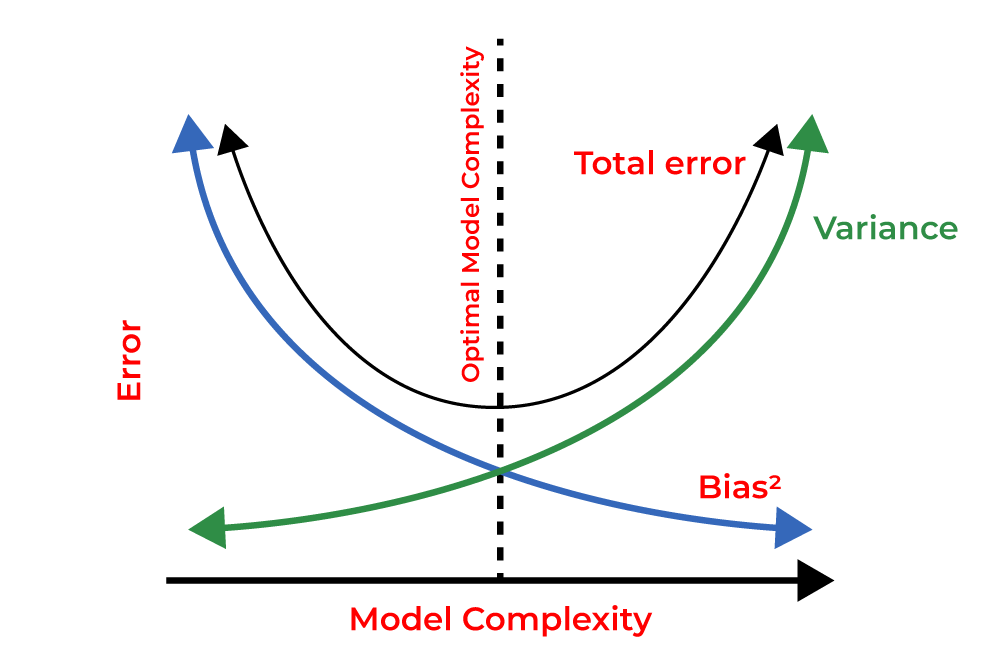
\includegraphics[scale=0.3]{notebooks/Others/img/bias_vs_variance.png}
    \caption{Bias vs Variance Diagram}
\end{figure}

\subsection{Oversampling and Undersampling}

\subsection{Random Noise Feature Importance}

\subsection{SHAP Values}
\label{subsec:shap_values}

El SHAP values (\textit{SHapley Additive exPlanations}) es un algoritmo modelo-agnóstico basado en teoría de juegos que permite \textbf{interpretar las predicciones}, la importancia de las variables y su impacto.

\begin{figure}[H]
    \center
    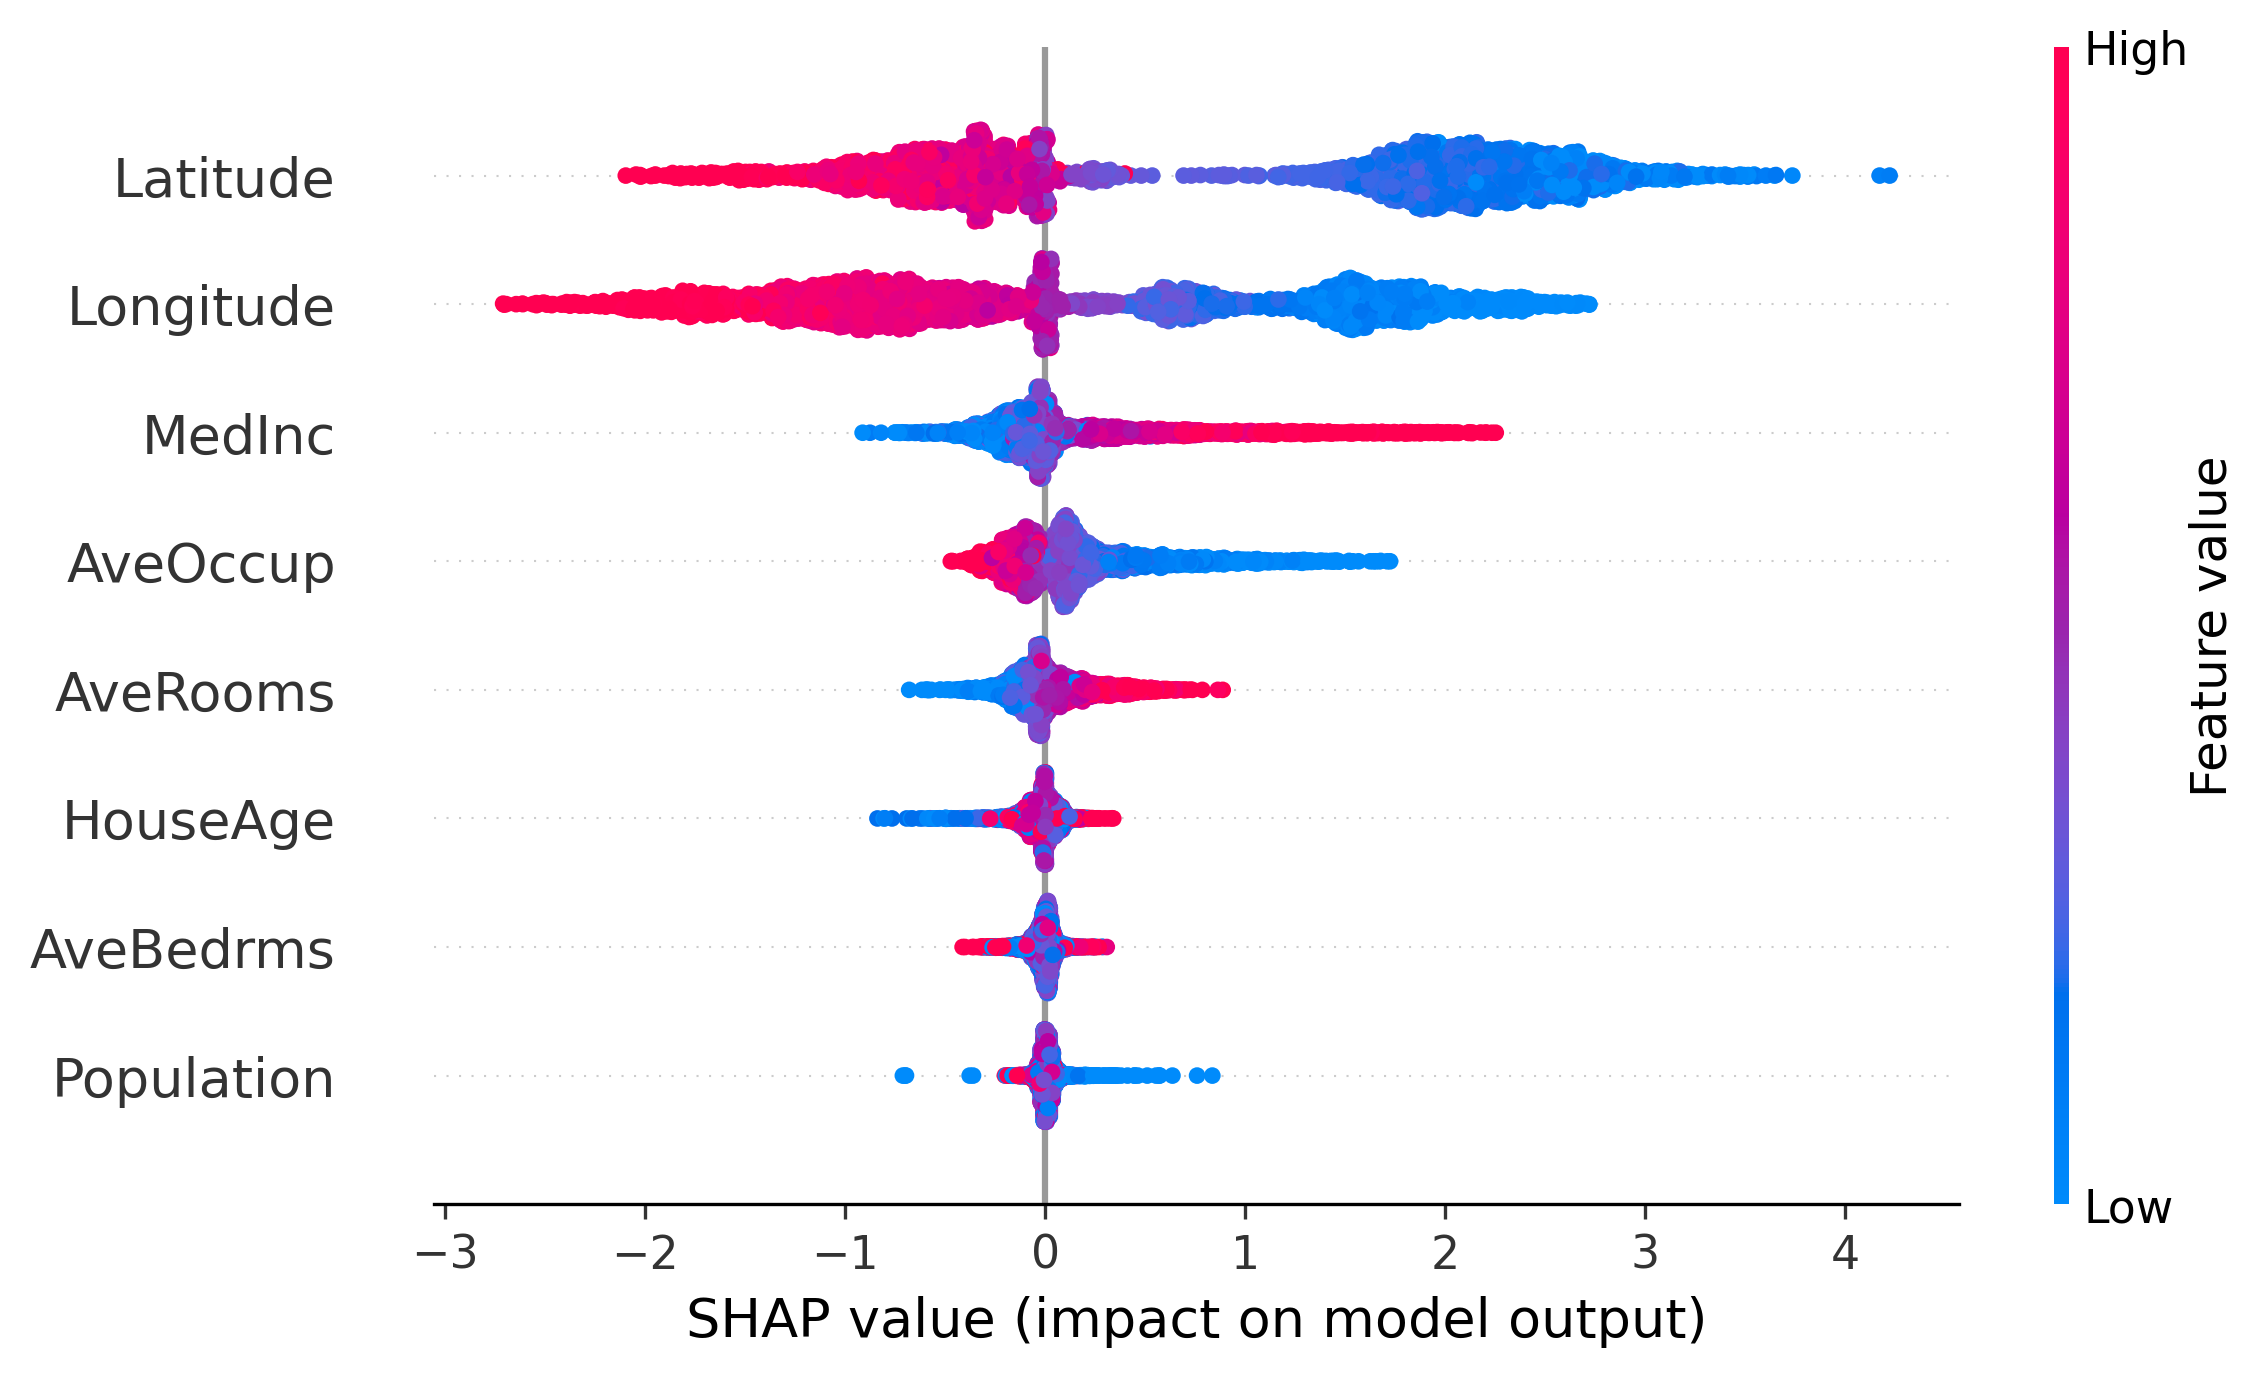
\includegraphics[scale=0.55]{notebooks/Others/img/shap_values_example.png}
    \caption{SHAP Values Example}
\end{figure}

\subsection{Cross-Validation Techniques}

El \textit{Cross-Validation} es un método que permite evaluar el rendimiento de un modelo de \textit{Machine Learning} y que busca eliminar el sesgo de la elección del conjunto de entrenamiento y testeo. Es ampliamente utilizado para la búsqueda de los mejores hiper-parámetros de un modelo. 


\begin{enumerate}
    \item \textbf{KFold}: Esta técnica consiste en dividir el conjunto de entrenamiento en $k$ partes. En cada iteración, se selecciona una de las particiones para testing y el resto para training. El score será el promedio de los scores obtenidos. Existe una variación llamada \textbf{StratifiedKFold} en la cual se asegura además que el \textit{target} tenga la misma distribución en cada partición test. 
    \item \textbf{ShuffleSplit}: Esta técnica selecciona la partición de entrenamiento y testing de manera aleatoria. No asegura que las particiones no sean las mismas en cada iteración. 
    \item \textbf{LeavePOut}: Esta técnica deja $p$ datos para el conjunto de testeo y entrena con todo el resto. Este proceso se realiza con todas las combinaciones posibles lo que asegura una estimación con menor \textit{bias} aunque es extremadamente ineficiente. 
\end{enumerate}

\begin{figure}[H]
    \center
    \includegraphics[scale=0.55]{notebooks/Others/img/}
    \caption{SHAP Values Example}
\end{figure}

\subsubsection{Time Series Cross Validation}

En el caso de series de tiempo, es importante notar que al momento de realizar \textit{Cross-Validation}, para problemas de \textit{Forecast} es importante \textbf{no entrenar con datos posteriores al testing} pues en la práctica, no se tendría acceso a estos.



\subsection{Outlier Detection}







